\chapter{Kimia Organologam: Ikatan dan Ligan}\label{ch:b3:organometallic-bonding}

Pada 1951 dua kelompok peneliti, secara terpisah, memperoleh serbuk jingga yang
stabil di udara dengan rumus $\ce{FeC10H10}$ yang tidak masuk akal: besi biasanya tidak
membentuk ikatan yang stabil dengan karbon, apalagi dengan dua cincin
siklopentadienil sekaligus. Dalam setahun strukturnya ditetapkan: besi terletak
di antara dua cincin yang sejajar dan terikat sama kuat pada kesepuluh atom
karbon, sebuah sandwich. Ferosena membuka kimia organologam modern, yang
katalis-katalisnya kini membuat sebagian besar polimer, obat, dan bahan kimia
halus dunia (\cref{ch:b3:homogeneous-catalysis}). Bab ini menjelaskan bagaimana
logam berikatan dengan karbon monoksida, fosfina, alkena, cincin, \omterm{def:b3:organometallic-bonding:carbene}{karbena}, dan
dengan sesamanya, serta bagaimana \omterm{def:b3:organometallic-bonding:isolobal}{analogi isolobal} menghubungkan
fragmen-fragmen organologam dengan kimia organik karbon.

\begin{recall}
Jilid Tahun 1 mendefinisikan senyawa organologam dan memakai pereaksi Grignard.
Jilid Tahun 2 memperkenalkan aturan 18 elektron dan penghitungan elektron
valensi, hapisitas, ligan akseptor $\pi$ dan donor $\pi$ beserta donasi balik, tahap-tahap
elementer reaksi organologam (adisi oksidatif, eliminasi reduktif,
insersi) dan orbital fragmen. \Cref{ch:b3:group-theory-applied} menghitung
uluran CO yang \omterm{def:b3:group-theory-applied:activity}{aktif IR} pada karbonil dan membangun kombinasi-kombinasi yang
teradaptasi simetri; \cref{ch:b3:complex-spectra-magnetism} mengaitkan momen
magnetik dengan elektron-elektron yang tidak berpasangan.
\end{recall}

\begin{omfigure}
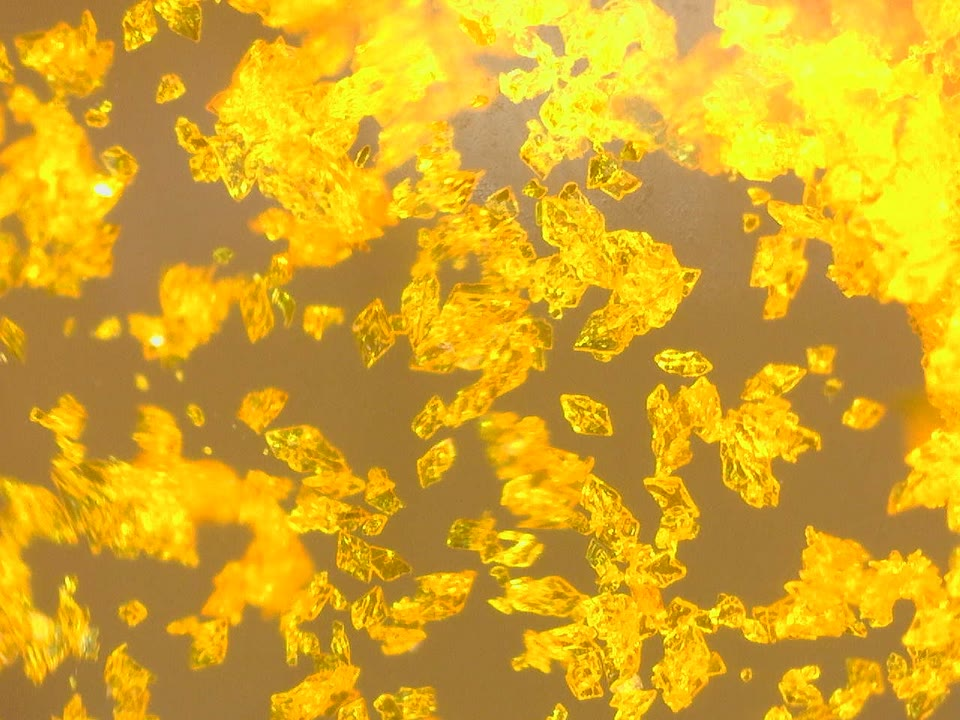
\includegraphics[width=0.5\linewidth]{images/book4/ferrocene-crystals.jpg}

{\small Kristal ferosena, $\ce{Fe(C5H5)2}$: senyawa organologam berwarna jingga yang
stabil di udara dan menyublim jika dihangatkan perlahan.}
\end{omfigure}

\section{Penghitungan elektron dan bilangan oksidasi}

\begin{method}[Menghitung elektron dengan dua cara]\label{met:b3:organometallic-bonding:count}
\begin{enumerate}
  \item Metode ligan netral (kovalen): logam menyumbang elektron sebanyak nomor
        golongannya; setiap ligan, yang dianggap netral, menyumbang 1 (H, \ce{CH3}, Cl,
        alil-$\eta^1$) atau 2 (CO, \ce{PR3}, alkena) atau lebih ($\eta^5$-\ce{C5H5} 5, $\eta^6$-\ce{C6H6} 6); tambahkan satu untuk setiap
        ikatan logam--logam dan koreksilah untuk muatan keseluruhan.
  \item Metode ionik: ligan seperti H, \ce{CH3}, Cl, \ce{C5H5} dihitung sebagai anion (2, 2,
        2, dan 6 elektron), dan logamnya sebagai kation $d^n$ yang dihasilkan; ligan netral
        dihitung seperti sebelumnya.
  \item Kedua metode memberikan jumlah total yang sama; metode ionik juga memberikan
        bilangan oksidasi dan jumlah $d^n$.
\end{enumerate}
\end{method}

\begin{example}[Penghitungan]\label{ex:b3:organometallic-bonding:count}
$\ce{Fe(CO)5}$: $8 + 5 \times 2 = 18$, besi(0), $d^8$. Ferosena: metode netral $8 + 2 \times 5 = 18$; metode ionik
$\ce{Fe^{2+}}$ ($d^6$, 6) $+ 2 \times 6$ ($\ce{C5H5-}$) $= 18$, besi(II). $\ce{Mn2(CO)10}$: setiap Mn $7 + 5 \times 2 + 1$ (ikatan
Mn--Mn) $= 18$. Kompleks $d^8$ segi empat datar seperti $\ce{[PtCl4]^{2-}}$ atau katalis Wilkinson
$\ce{RhCl(PPh3)3}$ memiliki 16 elektron: orbitalnya yang kosong dan mirip $p_z$ terlalu tinggi untuk diisi, dan
kompleks segi empat datar 16 elektron sama stabilnya dengan kompleks 18 elektron.
\end{example}

\section{Karbonil dan fosfina}

\begin{definition}[Karbonil logam]\label{def:b3:organometallic-bonding:carbonyl}
Yang disebut \emph{karbonil logam}\index{karbonil logam} adalah kompleks dengan ligan
karbon monoksida. Yang disebut \emph{karbonil terminal}\index{karbonil terminal} adalah karbonil yang terikat pada satu
logam melalui karbon; sedangkan \emph{karbonil penjembatan}\index{karbonil penjembatan}
merentang dua (atau tiga) logam.
\end{definition}

Pada 1890 Ludwig Mond mendapati bahwa nikel bereaksi dengan karbon monoksida
pada suhu biasa membentuk cairan atsiri $\ce{Ni(CO)4}$, yang terurai kembali menjadi nikel
murni jika dipanaskan: dasar sebuah proses pemurnian. Karbon monoksida mengikat
logam transisi melalui orbital terisi tertingginya, yaitu pasangan elektron bebas $\sigma$ yang sebagian besar
berada pada karbon, dan menerima elektron ke dalam orbital $\pi^*$-nya yang kosong, yang juga lebih besar pada
karbon.

\begin{definition}[Ikatan sinergis]\label{def:b3:organometallic-bonding:synergic}
Yang disebut \emph{ikatan sinergis}\index{ikatan sinergis} adalah saling penguatan antara
donasi $\sigma$ dari ligan ke logam dan donasi balik $\pi$ dari logam ke
ligan: donasi membuat logam lebih kaya elektron dan lebih siap untuk
mengembalikannya, sedangkan donasi balik meringankan muatan yang menumpuk akibat donasi.
\end{definition}

\begin{omfigure}
\begin{tikzpicture}[font=\small, >=Stealth]
  % donasi sigma
  \fill[black!70] (0,0) circle (0.14); \node[anchor=north] at (0,-0.4) {M};
  \pic at (0,0) {omlobe={-0.7}{180}};
  \pic at (0,0) {omlobe={0.9}{0}};
  \node[circle, fill=black!40, inner sep=1.6pt] at (1.9,0) {};
  \node[circle, fill=omThm!70, inner sep=1.6pt] at (3.0,0) {};
  \pic at (1.9,0) {omlobe={0.85}{180}};
  \node[font=\scriptsize, anchor=north] at (1.9,-0.25) {C};
  \node[font=\scriptsize, anchor=north] at (3.0,-0.25) {O};
  \draw[->, thick, omThm] (1.4,0.55) to[bend right=30] (0.6,0.55);
  \node[anchor=north] at (1.5,-1.55) {donasi $\sigma$};
  % donasi balik pi
  \begin{scope}[xshift=6.0cm]
    \fill[black!70] (0,0) circle (0.14); \node[anchor=north] at (0,-1.1) {M};
    \pic at (0,0) {omdxz};
    \node[circle, fill=black!40, inner sep=1.6pt] at (1.9,0) {};
    \node[circle, fill=omThm!70, inner sep=1.6pt] at (3.0,0) {};
    \pic at (1.9,0) {omp={0.9}{90}};
    \pic at (3.0,0) {omp={-0.6}{90}};
    \draw[->, thick, omThm] (0.6,1.05) to[bend left=30] (1.6,1.05);
    \node[anchor=north] at (1.5,-1.55) {donasi balik $\pi$};
  \end{scope}
\end{tikzpicture}

{\small \omterm{def:b3:organometallic-bonding:synergic}{Ikatan sinergis} karbon monoksida. Kiri: pasangan elektron bebas karbon (orbital $\sigma$)
berdonasi ke orbital logam bertipe $\sigma$ yang kosong. Kanan: orbital $d$ logam yang terisi
($d_{xz}$, dengan kedua sumbunya) bertumpang tindih dengan orbital $\pi^*$ CO yang kosong, yang lebih besar pada
karbon, yang cuping-cupingnya cocok dengan fasenya: elektron mengalir kembali ke orbital yang
bersifat antiikatan antara C dan O.}
\end{omfigure}

\begin{proposition}[Frekuensi uluran CO]\label{prop:b3:organometallic-bonding:co-frequency}
Makin banyak logam berdonasi balik ke orbital $\pi^*$ ligan CO, makin rendah
bilangan gelombang uluran C--O.
\end{proposition}

\begin{proof}[Argumen]
Orbital $\pi^*$ CO bersifat antiikatan antara C dan O: mengisinya melemahkan ikatan
C--O, menurunkan \omterm{def:b3:quantum-model-systems:oscillator}{tetapan gayanya}, dan karena itu bilangan gelombang uluran, yang
berubah sebanding dengan akar kuadrat \omterm{def:b3:quantum-model-systems:oscillator}{tetapan gaya} (\cref{ch:b3:rovibrational-spectroscopy}).
Donasi $\sigma$ mengambil elektron dari orbital yang hampir nonikatan (sedikit
antiikatan) untuk C--O, yang dengan sendirinya akan sedikit menaikkan bilangan gelombang: penurunan
yang teramati menunjukkan bahwa donasi balik mendominasi.
\end{proof}

Karbon monoksida bebas memiliki fundamental pada $\omega_e - 2\omega_ex_e = \qty{2143}{cm^{-1}}$; \omterm{def:b3:organometallic-bonding:carbonyl}{karbonil
terminal} kompleks netral menyerap kira-kira antara 1900 dan \qty{2100}{cm^{-1}},
\omterm{def:b3:organometallic-bonding:carbonyl}{karbonil penjembatan} lebih rendah lagi. Sepanjang deret isoelektronik, karbonil
anionik menyerap pada bilangan gelombang yang lebih rendah daripada karbonil netral, dan karbonil kationik pada
bilangan gelombang yang lebih tinggi: makin kaya elektron logamnya, makin banyak ia berdonasi balik. Jumlah
pita, berdasarkan simetri (\cref{ch:b3:group-theory-applied}), memberikan geometrinya.
% ledger: diat:CO.we, diat:CO.wexe

\begin{proposition}[Interaksi $\pi$ dan pembelahan medan ligan]\label{prop:b3:organometallic-bonding:pi-delta}
Dalam kompleks oktahedral, ligan akseptor $\pi$ menaikkan $\Delta_{\mathrm o}$ dan ligan donor $\pi$
menurunkannya.
\end{proposition}

\begin{proof}
Orbital-orbital $e_g$ hanya memiliki simetri $\sigma$. Orbital-orbital $t_{2g}$ ($d_{xy}$, $d_{xz}$, $d_{yz}$) cocok dengan kombinasi $t_{2g}$
orbital-orbital $\pi$ ligan: untuk $d_{xy}$, keempat ligan di bidang $xy$ masing-masing
menawarkan orbital $\pi$ yang tegak lurus terhadap sumbu M--L-nya di bidang itu, dan
kombinasi dengan tanda berselang-seling memiliki simetri $d_{xy}$ (kombinasi-kombinasi
lainnya bertransformasi sebagai $t_{1g}$, $t_{1u}$, dan $t_{2u}$ dan tidak menemukan pasangan $d$). Dua orbital dengan
simetri yang sama bercampur dan saling tolak: yang lebih rendah terdorong turun, yang lebih tinggi naik. Akseptor
$\pi$ menawarkan orbital kosong di atas himpunan $t_{2g}$, yang lalu terdorong turun: $\Delta_{\mathrm o}$
bertambah. Donor $\pi$ menawarkan orbital terisi di bawahnya, yang mendorongnya naik: $\Delta_{\mathrm o}$
berkurang. Tingkat $e_g$ tidak terpengaruh dalam kedua kasus.
\end{proof}

Itulah sebabnya CO dan \ce{CN-} berada di ujung kuat deret spektrokimia, sedangkan
halida dan hidroksida di ujung lemah, seperti yang dinyatakan Jilid Tahun 2.

\begin{definition}[Parameter Tolman]\label{def:b3:organometallic-bonding:tolman}
Yang disebut \emph{sudut kerucut Tolman}\index{sudut kerucut Tolman} sebuah fosfina adalah sudut
puncak kerucut, yang berpusat pada logam pada jarak standar, yang tepat
melingkupi permukaan van der Waals substituen-substituennya: sebuah ukuran besarnya.
Yang disebut \emph{parameter elektronik Tolman}\index{parameter elektronik Tolman} adalah
bilangan gelombang uluran CO simetris pada $\ce{Ni(CO)3L}$: makin kuat
fosfina L berdonasi, makin rendah nilainya.
\end{definition}

Fosfina dapat diatur ukuran dan donasi elektronnya secara terpisah melalui
substituennya: trialkilfosfina adalah donor yang lebih kuat daripada triarilfosfina,
dan fosfit yang paling lemah; $\ce{P(tBu)3}$ jauh lebih meruah daripada $\ce{PMe3}$. Fosfina yang meruah menyukai
bilangan koordinasi yang rendah dan disosiasi ligan yang cepat, dan itulah sebabnya fosfina semacam itu
muncul dalam begitu banyak katalis.

\section{Ligan $\pi$}

\begin{definition}[Model Dewar--Chatt--Duncanson]\label{def:b3:organometallic-bonding:dcd}
Yang disebut \emph{model Dewar--Chatt--Duncanson}\index{model Dewar--Chatt--Duncanson}
ikatan alkena pada logam adalah model yang memadukan donasi $\sigma$ dari orbital $\pi$ C=C
ke orbital logam yang kosong dengan donasi balik dari orbital $d$ logam yang terisi ke
orbital $\pi^*$ C=C. Limitnya untuk donasi balik yang kuat adalah sebuah
\emph{metalasiklopropana}\index{metalasiklopropana}, cincin beranggota tiga
dengan dua ikatan $\sigma$ M--C dan sebuah ikatan tunggal C--C.
\end{definition}

\begin{proposition}[Akibat donasi balik ke alkena]\label{prop:b3:organometallic-bonding:dcd}
Koordinasi memperpanjang ikatan C=C dan membengkokkan substituen-substituennya ke belakang, menjauhi
logam, makin besar ketika donasi baliknya makin kuat.
\end{proposition}

\begin{proof}[Argumen]
Mengambil elektron dari orbital $\pi$ (ikatan) dan menambahkannya ke orbital $\pi^*$
(antiikatan) sama-sama menurunkan orde ikatan C--C. Pencampuran karakter $\pi^*$
merehibridisasi karbon-karbonnya ke arah $sp^3$, yang ikatannya dengan substituen mengarah menjauhi
logam, menuju geometri \omterm{def:b3:organometallic-bonding:dcd}{metalasiklopropana}.
\end{proof}

\begin{omfigure}
\begin{tikzpicture}[font=\small, >=Stealth]
  \fill[black!70] (0,0) circle (0.14); \node[anchor=north] at (0,-1.1) {M};
  \pic at (0,0) {omlobe={0.9}{0}};
  \foreach \y in {0.45,-0.45}{\node[circle, fill=black!40, inner sep=1.6pt] at (1.9,\y) {};}
  \pic at (1.9,0.45) {omp={-0.75}{0}};
  \pic at (1.9,-0.45) {omp={-0.75}{0}};
  \draw[->, thick, omThm] (1.3,1.0) to[bend right=30] (0.5,0.6);
  \node[anchor=north] at (1.2,-1.4) {$\sigma$: $\pi$(C=C) $\to$ M};
  \begin{scope}[xshift=5.6cm]
    \fill[black!70] (0,0) circle (0.14); \node[anchor=north] at (0,-1.1) {M};
    \pic at (0,0) {omdxy};
    \foreach \y in {0.45,-0.45}{\node[circle, fill=black!40, inner sep=1.6pt] at (1.9,\y) {};}
    \pic at (1.9,0.45) {omp={-0.75}{0}};
    \pic at (1.9,-0.45) {omp={0.75}{0}};
    \draw[->, thick, omThm] (0.7,0.9) to[bend left=30] (1.5,0.9);
    \node[anchor=north] at (1.2,-1.4) {$\pi$: M $\to$ $\pi^*$(C=C)};
  \end{scope}
\end{tikzpicture}

{\small \omterm{def:b3:organometallic-bonding:dcd}{Model Dewar--Chatt--Duncanson} untuk alkena yang terikat dari samping (C=C
vertikal, logam di sebelah kiri). Kiri: orbital $\pi$ yang terisi (dua orbital $p$ yang
sefase) berdonasi ke orbital logam yang kosong. Kanan: orbital $d$ logam yang terisi
dengan fase yang cocok berdonasi ke orbital $\pi^*$ yang kosong (dua orbital $p$ yang
berlawanan fase).}
\end{omfigure}

Garam Zeise, $\ce{K[PtCl3(C2H4)]}$, yang dibuat pada 1827, adalah senyawa organologam pertama
dari logam transisi; etenanya terletak tegak lurus terhadap bidang \ce{PtCl3}, seperti
yang diramalkan model itu. Alil ($\eta^3$), diena ($\eta^4$), arena ($\eta^6$), dan cincin
siklopentadienil ($\eta^5$) terikat dengan cara yang sama melalui beberapa karbon sekaligus.

\begin{definition}[Metalosena]\label{def:b3:organometallic-bonding:metallocene}
Yang disebut \emph{senyawa sandwich}\index{senyawa sandwich} adalah senyawa yang logamnya
terletak di antara dua ligan cincin datar yang sejajar dan terikat melalui semua karbonnya; yang
disebut \emph{metalosena}\index{metalosena} adalah senyawa sandwich dengan dua cincin
siklopentadienil-$\eta^5$, $\ce{M(C5H5)2}$.
\end{definition}

\begin{proposition}[Orbital-orbital batas ferosena]\label{prop:b3:organometallic-bonding:ferrocene}
Dalam \omterm{def:b3:organometallic-bonding:metallocene}{metalosena} dengan cincin-cincin yang sejajar ($D_{5d}$), orbital $d$ logam terpecah menjadi $e_{2g}$
($d_{xy}$, $d_{x^2-y^2}$) dan $a_{1g}$ ($d_{z^2}$), yang hampir nonikatan dan berdekatan, serta $e_{1g}^\ast$ ($d_{xz}$,
$d_{yz}$), yang sangat antiikatan; ferosena, dengan enam elektron $d$ dalam $e_{2g}^4a_{1g}^2$, memiliki 18
elektron dan tidak memiliki elektron yang tidak berpasangan.
\end{proposition}

\begin{proof}[Argumen]
Orbital-orbital $\pi$ kedua cincin bergabung menjadi pasangan-pasangan yang teradaptasi simetri $a_{1g}$, $a_{2u}$,
$e_{1g}$, $e_{1u}$, $e_{2g}$, $e_{2u}$ (dari kelima orbital $\pi$ setiap cincin, dengan nol, satu, dan dua
bidang simpul yang melalui sumbu). Kombinasi cincin $e_{1g}$ yang terisi bertumpang tindih
kuat dengan $d_{xz}$, $d_{yz}$ (masing-masing satu bidang simpul melalui sumbu): keduanya membentuk orbital
ikatan, yang sebagian besar berkarakter cincin, dan orbital antiikatan $e_{1g}^\ast$, yang sebagian besar berkarakter logam dan terdorong tinggi. $d_{xy}$, $d_{x^2-y^2}$
(dua bidang simpul) hanya bertemu dengan orbital-orbital cincin $e_{2g}$ yang kosong dan sedikit
distabilkan oleh donasi balik; $d_{z^2}$ mengarah ke lubang di tengah setiap cincin dan
hampir tidak bertumpang tindih. Enam elektron mengisi $e_{2g}$ dan $a_{1g}$; bersama dua belas elektron
kombinasi cincin yang bersifat ikatan, jumlahnya 18.
\end{proof}

\begin{omfigure}
\begin{tikzpicture}[font=\small]
  % gambar sandwich
  \begin{scope}[xshift=-1.0cm]
    \draw[thick, fill=black!8] (0,1.0) ellipse (1.0 and 0.3);
    \draw[thick, fill=black!8] (0,-1.0) ellipse (1.0 and 0.3);
    \foreach \a in {90,162,234,306,18}{\fill[black!60] ({cos(\a)},{1.0+0.3*sin(\a)}) circle (0.07);
      \fill[black!60] ({cos(\a)},{-1.0+0.3*sin(\a)}) circle (0.07);}
    \shade[ball color=orange!70!brown] (0,0) circle (0.2);
    \node[anchor=west] at (0.25,0) {Fe};
  \end{scope}
  % diagram tingkat untuk empat metalosena
  \pic[transform shape] at (2.1,-0.9) {omlevel={u}{0.5}};
  \pic[transform shape] at (2.7,-0.9) {omlevel={ud}{0.5}};
  \pic[transform shape] at (2.4,-0.4) {omlevel={ud}{0.5}};
  \pic[transform shape] at (2.1,1.0) {omlevel={}{0.5}};
  \pic[transform shape] at (2.7,1.0) {omlevel={}{0.5}};
  \node[anchor=north] at (2.4,-1.3) {\ce{[FeCp2]+}};
  \node[anchor=north, font=\scriptsize] at (2.4,-1.75) {17 e$^-$};
  \pic[transform shape] at (4.3,-0.9) {omlevel={ud}{0.5}};
  \pic[transform shape] at (4.9,-0.9) {omlevel={ud}{0.5}};
  \pic[transform shape] at (4.6,-0.4) {omlevel={ud}{0.5}};
  \pic[transform shape] at (4.3,1.0) {omlevel={}{0.5}};
  \pic[transform shape] at (4.9,1.0) {omlevel={}{0.5}};
  \node[anchor=north] at (4.6,-1.3) {\ce{FeCp2}};
  \node[anchor=north, font=\scriptsize] at (4.6,-1.75) {18 e$^-$};
  \pic[transform shape] at (6.5,-0.9) {omlevel={ud}{0.5}};
  \pic[transform shape] at (7.1,-0.9) {omlevel={ud}{0.5}};
  \pic[transform shape] at (6.8,-0.4) {omlevel={ud}{0.5}};
  \pic[transform shape] at (6.5,1.0) {omlevel={u}{0.5}};
  \pic[transform shape] at (7.1,1.0) {omlevel={}{0.5}};
  \node[anchor=north] at (6.8,-1.3) {\ce{CoCp2}};
  \node[anchor=north, font=\scriptsize] at (6.8,-1.75) {19 e$^-$};
  \pic[transform shape] at (8.7,-0.9) {omlevel={ud}{0.5}};
  \pic[transform shape] at (9.3,-0.9) {omlevel={ud}{0.5}};
  \pic[transform shape] at (9.0,-0.4) {omlevel={ud}{0.5}};
  \pic[transform shape] at (8.7,1.0) {omlevel={u}{0.5}};
  \pic[transform shape] at (9.3,1.0) {omlevel={u}{0.5}};
  \node[anchor=north] at (9.0,-1.3) {\ce{NiCp2}};
  \node[anchor=north, font=\scriptsize] at (9.0,-1.75) {20 e$^-$};
  \node[anchor=east, font=\scriptsize] at (1.8,-0.9) {$e_{2g}$};
  \node[anchor=east, font=\scriptsize] at (1.8,-0.4) {$a_{1g}$};
  \node[anchor=east, font=\scriptsize] at (1.8,1.0) {$e_{1g}^\ast$};
\end{tikzpicture}

{\small Kiri: struktur sandwich ferosena (cincin-cincin eklips). Kanan:
orbital-orbital batas berbasis $d$ pada \omterm{def:b3:organometallic-bonding:metallocene}{metalosena}, $e_{2g}$ dan $a_{1g}$ yang hampir nonikatan, $e_{1g}^\ast$
yang antiikatan, yang terisi untuk kation ferosenium (17 elektron), ferosena (18),
kobaltosena (19), dan nikelosena (20, satu elektron di setiap orbital $e_{1g}^\ast$, dengan spin
sejajar menurut aturan Hund).}
\end{omfigure}

\section{Karbena, karbuna, dan ikatan logam--logam}

\begin{definition}[Karbena dan kompleks karbena]\label{def:b3:organometallic-bonding:carbene}
Yang disebut \emph{karbena}\index{karbena} adalah spesies netral $\ce{R2C}$ dengan karbon divalen
yang membawa dua elektron nonikatan. Yang disebut \emph{kompleks karbena}\index{kompleks karbena}
adalah kompleks yang memiliki ligan $\ce{CR2}$ yang terikat pada logam melalui ikatan rangkap, $\ce{M=CR2}$. Kompleks
\emph{karbena Fischer}\index{karbena Fischer} memiliki substituen heteroatom
pada karbon karbena dan logam bervalensi rendah dengan ligan akseptor $\pi$; karbon karbenanya
bersifat elektrofilik. Kompleks \emph{karbena Schrock}\index{karbena Schrock} (alkilidena)
hanya memiliki substituen C atau H dan logam awal bervalensi tinggi; karbonnya bersifat
nukleofilik. Yang disebut \emph{karbena N-heterosiklik}\index{karbena N-heterosiklik} adalah
karbena siklik yang diapit oleh dua atom nitrogen, yang stabil sebagai senyawa bebas dan merupakan ligan
donor $\sigma$ yang kuat.
\end{definition}

Kedua jenis \omterm{def:b3:organometallic-bonding:carbene}{kompleks karbena} berbeda dalam cara ikatan M=C dibagi.
Pada \omterm{def:b3:organometallic-bonding:carbene}{karbena Fischer}, \omterm{def:b3:organometallic-bonding:carbene}{karbena} singlet mendonorkan pasangan elektron bebasnya ke logam dan
menerima donasi balik ke orbital $p$-nya yang kosong, yang juga distabilkan oleh pasangan elektron bebas
heteroatom: karbonnya tetap miskin elektron dan diserang oleh nukleofil. Pada
\omterm{def:b3:organometallic-bonding:carbene}{karbena Schrock}, dua fragmen triplet, logam dan \omterm{def:b3:organometallic-bonding:carbene}{karbena}, membentuk ikatan kovalen $\sigma +
\pi$ yang terpolarisasi ke arah karbon: alkilidena itu berperilaku seperti ilida Wittig.

\begin{definition}[Kompleks karbuna]\label{def:b3:organometallic-bonding:carbyne}
Yang disebut \emph{kompleks karbuna}\index{kompleks karbuna} adalah kompleks yang memiliki ikatan rangkap tiga antara logam
dan karbon yang membawa satu substituen, $\ce{M#CR}$.
\end{definition}

\begin{definition}[Ikatan $\delta$, ikatan rangkap empat]\label{def:b3:organometallic-bonding:delta}
Yang disebut \emph{ikatan $\delta$}\index{ikatan delta@ikatan $\delta$} adalah ikatan yang orbitalnya memiliki dua bidang simpul
yang memuat sumbu antarinti, yang terbentuk oleh tumpang tindih muka-ke-muka dua orbital
$d$ seperti $d_{xy}$ dan $d_{xy}$. Yang disebut \emph{ikatan rangkap empat}\index{ikatan rangkap empat}
memadukan satu ikatan $\sigma$, dua ikatan $\pi$, dan satu ikatan $\delta$ antara dua atom logam.
\end{definition}

\begin{proposition}[{\omterm{def:b3:organometallic-bonding:delta}{Ikatan rangkap empat} $[\mathrm{Re_2Cl_8}]^{2-}$}]\label{prop:b3:organometallic-bonding:quadruple}
Dalam $\ce{[Re2Cl8]^{2-}}$ (dua \ce{Re^{III}}, masing-masing $d^4$), kedelapan elektron $d$ menempati $\sigma^2\pi^4\delta^2$: orde
ikatan 4, yang mensyaratkan susunan eklips kedua satuan \ce{ReCl4}.
\end{proposition}

\begin{proof}
Dengan $z$ sepanjang sumbu Re--Re dan atom-atom Cl sepanjang $\pm x$ dan $\pm y$ pada setiap Re, $d_{x^2-y^2}$
mengarah ke klorida dan dipakai dalam ikatan Re--Cl. Keempat orbital $d$ lainnya
pada setiap logam bertumpang tindih berpasangan: $d_{z^2}$ dengan $d_{z^2}$ sepanjang sumbu ($\sigma$), $d_{xz}$ dengan $d_{xz}$ dan $d_{yz}$
dengan $d_{yz}$ secara berdampingan ($\pi$, dua kali), $d_{xy}$ dengan $d_{xy}$ muka-ke-muka ($\delta$, yang paling lemah).
Delapan elektron mengisi keempat kombinasi ikatan. Memutar satu satuan sebesar $45^\circ$
terhadap $z$ mengubah $d_{xy}$-nya menjadi $d_{x^2-y^2}$, yang tumpang tindihnya dengan $d_{xy}$ yang lain nol karena
simetri: ikatan $\delta$, dan bersamanya preferensi susunan eklips, hilang. Ketiga
tumpang tindih lainnya simetris silindris atau besarnya tidak berubah.
\end{proof}

% ledger: geom:Re2Cl8.ReRe
Jarak Re--Re sebesar \qty{2.24}{\angstrom} pada garam kaliumnya sangat pendek untuk dua atom logam, dan klorida-klorida kedua paruhnya memang eklips, melawan
tolakan steriknya: ikatan $\delta$, selemah apa pun, menahannya di sana.

\begin{omfigure}
\tdplotsetmaincoords{58}{25}
\begin{tikzpicture}[tdplot_main_coords, font=\small, scale=1.15]
  \draw[thick, black!60] (0,0,0) -- (0,0,2.0);
  \foreach \z in {0,2.0}{
    \foreach \b in {0,90,180,270}{
      \draw[black!45] (0,0,\z) -- ({1.55*cos(\b)},{1.55*sin(\b)},\z);}
    \foreach \a/\s in {45/omphasepos, 135/omphaseneg, 225/omphasepos, 315/omphaseneg}{
      \path[\s, opacity=0.9] plot[domain=0:360, samples=48, smooth cycle]
        ({0.62*cos(\a)+0.55*cos(\x)*cos(\a)-0.26*sin(\x)*sin(\a)},
         {0.62*sin(\a)+0.55*cos(\x)*sin(\a)+0.26*sin(\x)*cos(\a)}, {\z});}
    \foreach \b in {0,90,180,270}{
      \node[circle, fill=green!45!black, inner sep=1.8pt] at ({1.55*cos(\b)},{1.55*sin(\b)},\z) {};}
    \shade[ball color=black!40] (0,0,\z) circle (0.14);}
  \node[anchor=east, xshift=-1.9cm] at (0,0,2.0) {Re};
  \node[anchor=east, xshift=-1.9cm] at (0,0,0) {Re};
\end{tikzpicture}

{\small Komponen $\delta$ \omterm{def:b3:organometallic-bonding:delta}{ikatan rangkap empat} $\ce{[Re2Cl8]^{2-}}$: orbital-orbital $d_{xy}$
kedua atom renium (masing-masing empat cuping, tanda biru dan jingga) saling berhadapan
melintasi sumbu Re--Re, cuping di atas cuping yang tandanya sama. Klorida-klorida (hijau),
yang eklips, terletak sepanjang $x$ dan $y$, di antara cuping-cuping.}
\end{omfigure}

\section{Analogi isolobal}

\begin{definition}[Fragmen isolobal]\label{def:b3:organometallic-bonding:isolobal}
Dua fragmen molekul disebut \emph{isolobal}\index{fragmen isolobal} jika
jumlah, simetri, perkiraan energi, dan bentuk orbital-orbital batasnya, serta
jumlah elektron di dalamnya, serupa. Yang disebut \emph{analogi
isolobal}\index{analogi isolobal} adalah prinsip yang meramalkan bahwa fragmen-fragmen isolobal dapat saling
menggantikan dalam molekul.
\end{definition}

\begin{proposition}[Deret isolobal]\label{prop:b3:organometallic-bonding:isolobal}
$\ce{CH3}$, $\ce{Mn(CO)5}$, dan $\ce{CpFe(CO)2}$ \omterm{def:b3:organometallic-bonding:isolobal}{isolobal} (satu orbital batas, satu elektron);
demikian pula $\ce{CH2}$ dan $\ce{Fe(CO)4}$ (dua orbital, dua elektron), serta $\ce{CH}$ dan $\ce{Co(CO)3}$ (tiga orbital,
tiga elektron).
\end{proposition}

\begin{proof}[Argumen]
$\ce{CH3}$ adalah fragmen tetrahedral yang kehilangan satu ikatan: satu orbital mirip $sp^3$ dengan satu
elektron, kurang satu dari oktet. $\ce{Mn(CO)5}$ adalah oktahedron yang kehilangan satu ligan:
situs yang kosong memuat satu orbital hibrida yang mengarah ke luar; dengan $7 + 10 = 17$ elektron, fragmen itu kurang satu
dari 18, dan elektron tunggalnya menempati hibrida itu. Melepaskan dua atau tiga
ligan (atau ikatan) memberikan dua atau tiga orbital dan elektron semacam itu, dengan
penghitungan yang sama pada kedua sisi: $\ce{Fe(CO)4}$ memiliki 16 elektron ($8 + 8$), kurang dua dari 18;
$\ce{Co(CO)3}$ memiliki 15 ($9 + 6$), kurang tiga.
\end{proof}

\begin{method}[Meramalkan struktur dengan penggantian isolobal]\label{met:b3:organometallic-bonding:isolobal}
\begin{enumerate}
  \item Pecahlah senyawa itu menjadi fragmen-fragmen dan hitunglah orbital batas
        dan elektron setiap fragmen.
  \item Gantilah setiap fragmen dengan pasangan \omterm{def:b3:organometallic-bonding:isolobal}{isolobal} organiknya.
  \item Analog organiknya, jika ada, menyarankan ikatan dan bentuknya:
        $\ce{Mn2(CO)10}$ adalah ``etana'', $\ce{Co3(CO)9CH}$ adalah ``tetrahedrana'' $\ce{(CH)4}$ yang tiga CH-nya
        diganti dengan $\ce{Co(CO)3}$.
\end{enumerate}
\end{method}

\begin{omfigure}
\begin{tikzpicture}[font=\small]
  \foreach \y/\l/\r/\n in {0/{\ce{CH3}}/{\ce{Mn(CO)5}}/1, -1.6/{\ce{CH2}}/{\ce{Fe(CO)4}}/2, -3.2/{\ce{CH}}/{\ce{Co(CO)3}}/3}{
    \node at (0,\y) {\l};
    \node at (5.2,\y) {\r};
    \node[font=\large] at (2.6,\y) {$\longleftrightarrow$};
    \node[font=\scriptsize, anchor=south] at (2.6,\y+0.15) {isolobal};
    \node[font=\scriptsize, anchor=west] at (7.0,\y) {\ifnum\n=1 satu orbital batas, satu elektron\else\ifnum\n=2 dua orbital batas, dua elektron\else tiga orbital batas, tiga elektron\fi\fi};}
  \foreach \a in {0}{\pic at (0.55,0) {omlobe={0.6}{0}};}
  \pic at (6.25,0) {omlobe={0.6}{0}};
  \pic at (0.45,-1.6) {omlobe={0.6}{20}}; \pic at (0.45,-1.6) {omlobe={0.6}{-20}};
  \pic at (6.15,-1.6) {omlobe={0.6}{20}}; \pic at (6.15,-1.6) {omlobe={0.6}{-20}};
  \foreach \t in {-30,0,30}{\pic at (0.4,-3.2) {omlobe={0.55}{\t}}; \pic at (6.1,-3.2) {omlobe={0.55}{\t}};}
\end{tikzpicture}

{\small Deret \omterm{def:b3:organometallic-bonding:isolobal}{isolobal} (hibrida-hibrida batas digambar secara skematis): setiap fragmen
organik dan fragmen \omterm{def:b3:organometallic-bonding:carbonyl}{karbonil logam} di seberangnya memiliki jumlah orbital batas yang mengarah
ke luar dan jumlah elektron di dalamnya yang sama, dan bergabung dengan
cara-cara yang analog.}
\end{omfigure}

\begin{definition}[Interaksi agostik]\label{def:b3:organometallic-bonding:agostic}
Yang disebut \emph{interaksi agostik}\index{interaksi agostik} adalah ikatan tiga pusat
dua elektron antara logam dan ikatan C--H salah satu ligannya sendiri, tempat
pasangan elektron ikatan C--H berdonasi ke orbital logam yang kosong.
\end{definition}

Hidrogen agostik tampak sebagai jarak logam--hidrogen yang pendek dalam struktur
difraksi, sebagai bilangan gelombang uluran C--H yang luar biasa rendah, dan dalam NMR sebagai
geseran medan tinggi dan kopling $^1J_{\mathrm{CH}}$ yang berkurang. Interaksi itu merupakan potret beku
aktivasi C--H, tahap pertama banyak reaksi katalitik.

\begin{inthelab}[Bekerja dengan karbonil logam]
\omterm{def:b3:organometallic-bonding:carbonyl}{Karbonil logam} ditangani di dalam lemari asam dengan pengisapan yang berfungsi, di bawah
nitrogen atau argon, tanpa nyala terbuka: banyak di antaranya melepaskan karbon monoksida jika
dihangatkan. Karbonil yang atsiri dipindahkan dengan kanula atau pada jalur vakum, tidak pernah
dituang; residunya dimusnahkan dengan oksidasi lambat (pemutih atau air brom) di dalam
lemari asam. Nikel tetrakarbonil, yang paling berbahaya, sama sekali tidak dipakai di laboratorium
pengajaran.
\end{inthelab}

\begin{safety}{\ghs[0.62cm]{GHS02}\ghs[0.62cm]{GHS06}\ghs[0.62cm]{GHS07}\ghs[0.62cm]{GHS08}\ghs[0.62cm]{GHS09}}
% ledger: ghs4:NiCO4, ghs4:ferrocene
Nikel tetrakarbonil: sangat mudah menyala, fatal jika terhirup, diduga karsinogen,
dapat merusak janin. Ferosena: padatan mudah menyala, berbahaya jika tertelan;
ditangani sebagai bahan kimia halus dengan sarung tangan dan tindakan pencegahan debu.
\end{safety}

\begin{history}[Karbonil Mond dan sandwich]
Ludwig Mond dan rekan-rekan kerjanya menemukan nikel tetrakarbonil pada 1890 ketika
mempelajari korosi katup nikel oleh karbon monoksida, dan di atasnya membangun
sebuah proses pemurnian nikel. Ferosena dibuat pada 1951 oleh Thomas Kealy dan Peter
Pauson, dan secara terpisah oleh Samuel Miller, John Tebboth, dan John Tremaine; pada 1952
Geoffrey Wilkinson dan Robert Woodward, serta Ernst Otto Fischer, mengusulkan
struktur sandwich. Fischer dan Wilkinson berbagi Hadiah Nobel Kimia 1973 untuk
karya mereka tentang \omterm{def:b3:organometallic-bonding:metallocene}{senyawa sandwich}.
\end{history}

\section{Latihan}

\begin{exercise}[$\star$]\label{exo:b3:organometallic-bonding:1}
Hitunglah elektron valensi $\ce{Fe(CO)5}$, $\ce{Mn2(CO)10}$ (per Mn), $\ce{CpMo(CO)3H}$, anion Zeise
$\ce{[PtCl3(C2H4)]-}$, $\ce{Cr($\eta^6$-C6H6)(CO)3}$, dan $\ce{Cp2ZrCl2}$.
\end{exercise}

\begin{exercise}[$\star$]\label{exo:b3:organometallic-bonding:2}
Berikan bilangan oksidasi dan jumlah $d^n$ logam dalam setiap senyawa pada
latihan sebelumnya.
\end{exercise}

\begin{exercise}[$\star$]\label{exo:b3:organometallic-bonding:3}
Urutkan bilangan gelombang uluran CO $\ce{[V(CO)6]-}$, $\ce{Cr(CO)6}$, dan $\ce{[Mn(CO)6]+}$, lalu berikan alasannya.
\end{exercise}

\begin{exercise}[$\star$]\label{exo:b3:organometallic-bonding:4}
Berikan analog \omterm{def:b3:organometallic-bonding:isolobal}{isolobal} organik $\ce{Mn2(CO)10}$, $\ce{[CpFe(CO)2]2}$, dan $\ce{Co3(CO)9CH}$.
\end{exercise}

\begin{exercise}[$\star\star$]\label{exo:b3:organometallic-bonding:5}
Berapa banyak pita uluran CO yang diperlihatkan $fac$- dan $mer$-$\ce{M(CO)3L3}$ dalam IR?
\end{exercise}

\begin{exercise}[$\star\star$]\label{exo:b3:organometallic-bonding:6}
Jelaskan mengapa penggantian $\ce{PMe3}$ dengan $\ce{P(tBu)3}$ dalam sebuah katalis dapat mempercepat tahap yang memerlukan
lepasnya sebuah ligan dari logam.
\end{exercise}

\begin{exercise}[$\star\star$]\label{exo:b3:organometallic-bonding:7}
Golongkan $\ce{(CO)5Cr=C(OMe)Ph}$ dan $\ce{Ta(=CHCMe3)(CH2CMe3)3}$ sebagai \omterm{def:b3:organometallic-bonding:carbene}{kompleks karbena} Fischer atau
Schrock, dan ramalkan reaksinya dengan sebuah amina dan dengan sebuah keton.
\end{exercise}

\begin{exercise}[$\star\star$]\label{exo:b3:organometallic-bonding:8}
Berapakah orde ikatan $\ce{[Re2Cl8]^{2-}}$ dalam konformasi goyang? Berapakah orde ikatan
$\ce{[Re2Cl8]^{4-}}$, yang memiliki dua elektron lebih banyak?
\end{exercise}

\begin{exercise}[$\star\star$]\label{exo:b3:organometallic-bonding:9}
Sebutkan tiga jenis bukti untuk interaksi C--H agostik.
\end{exercise}

\begin{exercise}[$\star\star\star$]\label{exo:b3:organometallic-bonding:10}
Berikan contoh kompleks stabil dengan 16, 17, dan 19 elektron valensi, dan jelaskan
setiap penyimpangan dari aturan 18 elektron itu.
\end{exercise}

\begin{exercise}[$\star\star\star$]\label{exo:b3:organometallic-bonding:11}
$\ce{Cr(CO)6}$ tidak berwarna dan diamagnetik. Dengan efek akseptor $\pi$ pada $\Delta_{\mathrm o}$, jelaskan
mengapa senyawa itu berspin rendah dan mengapa pita-pita $d$--$d$-nya terletak di daerah ultraviolet.
\end{exercise}

\begin{exercise}[$\star\star\star$]\label{exo:b3:organometallic-bonding:12}
Ikatan C--C etena memanjang dari \qty{1.34}{\angstrom} menjadi \qty{1.37}{\angstrom} dalam garam Zeise dan menjadi
sekitar \qty{1.43}{\angstrom} dalam kompleks logam bervalensi rendah dengan donasi balik yang kuat (data
latihan). Tafsirkan dengan \omterm{def:b3:organometallic-bonding:dcd}{model Dewar--Chatt--Duncanson}.
\end{exercise}

\section{Soal: Sandwich}

\begin{problem}[{Soal akhir pekan --- sandwich: penghitungan elektron empat
metalosena, orbital-orbital batas dan elektron-elektron tak berpasangannya, kimia
redoksnya, serta dua pertanyaan tentang isolobalitas dan spektroskopi}]
\label{pb:b3:organometallic-bonding:1}
\omterm{def:b3:organometallic-bonding:metallocene}{Metalosena} $\ce{MCp2}$ ($\ce{Cp} = \eta^5$-$\ce{C5H5}$) dikenal untuk M = Fe, Co, Ni, dan untuk kation ferosenium.

\medskip\noindent\textbf{Bagian I --- Penghitungan.}
\begin{enumerate}[beginpenalty=10000]
  \item Hitunglah elektron ferosena dengan metode ionik.
  \item Hitunglah elektron itu dengan metode netral.
  \item Hitunglah elektron kobaltosena.
  \item Hitunglah elektron nikelosena.
  \item Hitunglah elektron kation ferosenium.
  \item Berikan bilangan oksidasi dan jumlah $d^n$ setiap logam.
\end{enumerate}

\medskip\noindent\textbf{Bagian II --- Orbital dan kemagnetan.}
\begin{enumerate}[resume, beginpenalty=10000]
  \item Golongkan kelima orbital $d$ dalam $D_{5d}$.
  \item Orbital manakah yang bertumpang tindih kuat dengan orbital $\pi$ cincin, dan dengan akibat
        apa?
  \item Berikan urutan tingkat-tingkat yang berbasis $d$.
  \item Isilah tingkat-tingkat itu untuk ferosena: berapa elektron yang tidak berpasangan?
  \item Isilah untuk kobaltosena: berapa elektron yang tidak berpasangan, dan berapa \omterm{def:b3:complex-spectra-magnetism:moment}{momen spin sajanya}?
  \item Isilah untuk nikelosena: berapa elektron yang tidak berpasangan, dan berapa \omterm{def:b3:complex-spectra-magnetism:moment}{momen spin sajanya}?
  \item Isilah untuk ferosenium: berapa elektron yang tidak berpasangan? Mengapa momen terukurnya
        di atas nilai spin saja?
\end{enumerate}

\medskip\noindent\textbf{Bagian III --- Redoks.}
\begin{enumerate}[resume, beginpenalty=10000]
  \item Mengapa kobaltosena merupakan reduktor yang kuat?
  \item Mengapa pasangan ferosena/ferosenium cepat dan reversibel?
  \item Mengapa pasangan itu dipakai sebagai acuan internal dalam elektrokimia nonair
        (\cref{ch:b3:electrode-kinetics})?
  \item Apakah yang dapat diharapkan dari reaksi nikelosena dengan ligan
        dua elektron?
\end{enumerate}

\medskip\noindent\textbf{Bagian IV --- Fragmen dan spektrum.}
\begin{enumerate}[resume, beginpenalty=10000]
  \item Tunjukkan bahwa $\ce{CpFe(CO)2}$ \omterm{def:b3:organometallic-bonding:isolobal}{isolobal} dengan \ce{CH3}, dan ramalkan struktur
        $\ce{[CpFe(CO)2]2}$.
  \item Dimer campuran apakah yang dapat dibentuknya dengan $\ce{Mn(CO)5}$?
  \item Bagaimana penggantian satu CO pada $\ce{CpMn(CO)3}$ dengan $\ce{PPh3}$ mengubah uluran CO
        yang tersisa?
  \item Berapa banyak pita CO yang diperlihatkan $\ce{Cr($\eta^6$-C6H6)(CO)3}$ ($C_{3v}$)?
  \item Mengapa cincin Cp-$\eta^5$ dapat bergeser menjadi $\eta^3$ selama substitusi?
  \item Nyatakan hasilnya: momen magnetik spin saja nikelosena.
\end{enumerate}
\end{problem}
